\section{Probleem Analyse en Eisen} \label{sec:ProbleemAnalyseEnEisen}

In deze sectie worden de beperkingen van de huidige testopstelling opgesomt en waarom deze beperkingen momenteel een probleem vormen.

\subsection{Huidige Situatie}

In de testkast zit de \gls{AX5140} \cite{web:AX5140Drive} servo drive geïnstalleerd (Figuur \ref{fig:AX5140}). Deze drive is uitgebreidt met een \gls{AX5801}-0200 \cite{web:AX5801} veiligheidskaart waardoor het mogelijk is om veiligheids functies zoals Safe Torque Off (\gls{STO}) te configureren om veilig (en snel) tot stilstand te komen.

\vspace{0.5cm}

De \gls{AX5140} servo drive ondersteunt standaard niet alle encoder protocollen en is daarom uit uitgebreid met de \gls{AX5701} \cite{web:AX5701} Encoder optie kaart zodat bijvoorbeeld EnDat en Hiperface encoders ook aangesloten kunnen worden.

\vspace{0.5cm}

Het testprogramma die momenteel op de testkast staat bevat maar één parameter set voor één type motor. Zelfs wanneer er meer parameter sets aanwezig zouden zijn is er in het huidige programma geen manier om deze automatisch te schrijven naar de drive heen. Nieuwe parametersets zullen handmatig met \gls{TwinCAT} XAE \cite{web:DriveManager2} naar de drive moeten worden geschreven. Dit kan tijdsintensief zijn en lastig zijn voor mensen die dit nooit eerder gedaan hebben het is daarom wenselijk om dit zo makkelijk mogelijk te maken.

\begin{figure}[h]
	\centering
	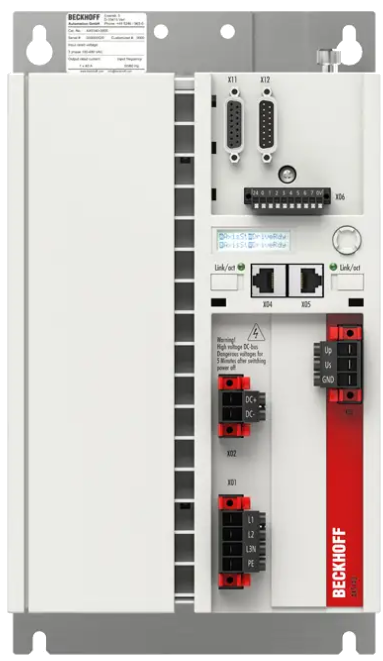
\includegraphics[width=150pt]{AX5140}
	\label{fig:AX5140}
	\caption{De \gls{AX5140} motordrive \cite{web:AX5140Drive}}
\end{figure}

\newpage

\subsection{Eisen}

Hieronder staan de belangrijkste eisen van de testopstelling van dit onderzoek. Voor alle eisen wordt doorverwezen naar het SRD bestand van de testopstelling (bijlage \ref{sec:TestKastSRD}).

\vspace{0.5cm}

\begin{table}[ht]
	\caption{FR-001 Geautomatiseerd testen}
	\label{tab:FR-001}
	\centering
	\begin{tabular}{|p{0.15\linewidth}|p{0.75\linewidth}|}
		\hline
		FR-001 & Geautomatiseerd testen URGENT \\
		
		\hline
		
		Stelling & De testkast moet in staat zijn om geautomatiseerd te kunnen testen. Dit houdt in dat er testen gemaakt moeten kunnen worden die vervolgens uitgevoerd kunnen worden op de testkast.\\
		
		Meetmethode & De eis is behaald wanneer een operator, die los staat van dit project, op de testkast een test kan maken met het instructieboekje en deze ook kan afspelen op de testkast. Deze testkast moet deze test dan automatisch afspelen. \\
		
		Opmerking & De operator moet tenminste de keuze hebben uit welk toerental, hoe snel de spindel deze moet bereiken en voor hoelang de spindel moet draaien in dit toerental. \\
		\hline
	\end{tabular}
\end{table}

\vspace{0.5cm}

\begin{table}[ht]
	\caption{FR-006 Automatisch parameters inladen}
	\label{tab:FR-006}
	\centering
	\begin{tabular}{|p{0.15\linewidth}|p{0.75\linewidth}|}
		\hline
		FR-006 & Automatisch parameters inladen URGENT \\
		
		\hline
		
		Stelling & De testkast moet geautomatiseerd andere parameters in kunnen laden van andere motoren.\\
		
		Meetmethode & De eis is behaald op het moment dat er een andere motor wordt aangesloten dat de gebruiker slechts door de motor te selecteren in de GUI de parameters kan inladen in de drive die passen bij die motor. \\
		
		Opmerking &  \\
		\hline
	\end{tabular}
\end{table}

\newpage

\begin{table}[ht]
	\caption{FR-007 Handmatig testen}
	\label{tab:FR-007}
	\centering
	\begin{tabular}{|p{0.15\linewidth}|p{0.75\linewidth}|}
		\hline
		FR-007 & Handmatig testen URGENT \\
		
		\hline
		
		Stelling & De gebruiker moet de spindels handmatig kunnen aansturen met de \gls{gui} op de testkast. \\
		
		Meetmethode & Deze eis is behaald wanneer de gebruiker handmatig de motor kan aansturen met de GUI op de testkast. \\
		
		Opmerking & Het aansturen kan bijvoorbeeld met een slider. \\
		\hline
	\end{tabular}
\end{table}

\newpage

\begin{table}[ht]
	\caption{FR-009 Handmatig testen}
	\label{tab:FR-009}
	\centering
	\begin{tabular}{|p{0.15\linewidth}|p{0.75\linewidth}|}
		\hline
		FR-009 & Servo Motoren URGENT \\
		
		\hline
		
		Stelling & Tenminste de volgende motoren moeten kunnen worden aangestuurd door de AX5140 motordrive:
		\begin{enumerate}
			\item MAD100D-0250-SA-C0-AK0-35-N3 (V623) Async servo motor
			\item MAD130C-0150-SA-S2-AP0-05-N1 (V633, V310 nieuw) Async servo motor
			\item HQL100X (V310 oud) Async servo motor
			\item MSK101D-0450-NN-M1-AP0-NNNN (V505-250T, V320, V330C, V320C en V600) Sync servo motor
			\item MS2N10-D0BNN-AMVK0-NNNNN-NN (V630 nieuw)  Sync servo motor
		\end{enumerate} \\
		
		Meetmethode & Deze eis is behaald wanneer bovenstaande motoren aangestuurd kunnen worden vanaf de drive de motoren moeten hierbij draaien. \\
		
		Opmerking & Het aansturen kan bijvoorbeeld met een slider. \\
		\hline
	\end{tabular}
\end{table}

\newpage

\begin{table}[ht]
	\caption{HR-004 Montage gaten}
	\label{tab:HR-004}
	\centering
	\begin{tabular}{|p{0.15\linewidth}|p{0.75\linewidth}|}
		\hline
		HR-004 & Montage gaten URGENT \\
		
		\hline
		
		Stelling & Alle spindels die Voortman wil gaan testen op de testkast moeten op de testkast kunnen dit houdt in dat de montage plaat verschillende gaten patronen moet hebben zodat alle spindels vastgemaakt kunnen worden aan de kast. \\
		
		Meetmethode & Deze eis is behaald op het moment dat de volgende motoren op de testkast kunnen worden gemonteerd met dezelfde gaten als wanneer deze op de machine zijn gemonteerd:
		\begin{enumerate}
			\item 007-5744 V6xx-DP Asm Drill spindle + motor DU1
			\item 009-2953 V623 Drill spindle DU1
			\item 009-2627 V623 Drill spindle DU2
			\item 009-3521 V623 Drill spindle DU3
			\item 005-6928 Drilling head
			\item 000-1744 Drilling head
			\item 009-7863 Drilling head Top
		\end{enumerate} \\
		
		Opmerking & Het aansturen kan bijvoorbeeld met een slider. \\
		\hline
	\end{tabular}
\end{table}


